\chapter{El algoritmo}

% TODO: escribir la idea general

\noindent
En este capítulo desarrollamos el algoritmo para resolver prácticamente cualquier tipo de problemas
de programación lineal entera; se divide en tres subsecciones que construyen el algoritmo de forma
incremental. En primer lugar, consideramos el caso cuando las únicas dos restricciones son de no
negatividad ($\vec{x} \geq \vec{0}$) y una presupuestaria ($\vec{c}^T\vec{x} \leq u$ para algún
escalar $u$). A partir de ello, generamos una sucesión de ecuaciones lineales enteras cuya solución
provee candidatos para el óptimo del problema.

En segundo lugar, agregamos $m$ restricciones de desigualdad además de la presupuestaria. Este es el
parteaguas donde el algoritmo toma relevancia, pero donde también aumenta en complejidad y supone
ciertas dificultades con los tiempos de terminación. Discutiremos ampliamente posibles direcciones
que puedan mejorar de manera significativa la rapidez de nuestro algoritmo.

En tercer lugar, eliminamos la restricción presupuestaria y, por lo tanto, nuestro algoritmo será
capaz de resolver problemas lineales enteros en su forma general. Ciertamente esta subsección es
la más corta, pues lo único que hacemos es agregar implícitamente una restricción presupuestaria
válida resolviendo el problema lineal relajado. Es de esta manera que podremos hacer uso de los
resultados obtenidos en la segunda fase.

En cuarto lugar, agregamos consideraciones que facilitan la implementación del algoritmo. En
particular, consideramos el caso donde hay una o más restricciones de igualdad, así como el caso
donde las variables de decisión son binarias. Finalmente, discutiremos brevemente una extensión a
este algoritmo para que sea capaz de resolver problemas lineales mixtos.

\begin{definition}[\cite{herr}]
	Decimos que un vector $\vec{v} \in \R^n \setminus \lbrace 0 \rbrace$ es esencialmente
	entero\footnote{El artículo los nombra \textit{projectively rational vectors}, mas el autor de
	esta tesis no encontró una traducción al español establecida, por lo que decidió nombrarlos de
	la forma que lo hizo. Por la misma razón, el autor decidió traducir \textit{c-layer} como ``capa
	entera'' en la Definición \ref{phase-1:def:c-layer}.} si existen $\vec{w} \in \Z^n$, $k \in \R$ tal
	que $\vec{v} = k\vec{w}$. Además, decimos que $\vec{w}$ es el múltiplo coprimo de $\vec{v}$ si sus
	entradas son coprimas (c.f. \ref{prerreq:def:gcd}) y si su primera entrada es no negativa.
\end{definition}

\noindent
En otras palabras, decimos que $\vec{v}$ es esencialmente entero si es un múltiplo real de un vector
entero.
\begin{example}
	El vector $\left(-\sqrt{2}, 1/\sqrt{2}\right)^T = \sqrt{2}(-1, 1/2)^T$ es esencialmente entero
	y $(2, -1)^T$ es su múltiplo coprimo. Contrariamente, el vector $(\sqrt{2}, \sqrt{3})^T$ no es
	esencialmente entero.
\end{example}

\begin{observation}
	Todo vector $\vec{v}$ cuyas entradas son racionales ($\vec{v} \in \Q^n$) es esencialmente
	entero. En efecto, $\vec{v}_i = \frac{p_i}{q_i}$ para algunos enteros $p_i$ y $q_i$ con $q_i$
	distinto de cero. Si definimos $q \coloneq \lcm{q_1, \ldots, q_n} \neq 0$ y $\vec{w} \coloneq
	q\vec{v}$, se sigue que $\vec{v} = \frac{1}{q}\vec{w}$ y también $\vec{w} \in \Z^n$.
\end{observation}

\begin{observation}
	Todo vector $\vec{v}$ esencialmente entero tiene a lo más dos vectores coprimos asociados. Sean
	$k \in \R$ y $\vec{w} \in \Z^n$ tales que $\vec{v} = k\vec{w}$. Entonces
	\begin{equation*}
		\pm \frac{1}{\gcd{\vec{w}_1, \ldots, \vec{w}_n}}\vec{w}
	\end{equation*}
	son dos vectores cuyas entradas son coprimas, de acuerdo al Corolario \ref{prerreq:cor:gcd}. Si
	$\vec{w}_1 = 0$, estos representan el mismo vector, y si $\vec{w}_1 \neq 0$ entonces solo uno de
	estos dos vectores es el múltiplo coprimo de $\vec{v}$. Independientemente del caso, el múltiplo
	coprimo de todo vector esencialmente entero es único.
\end{observation}

Porque todo número representable en cualquier sistema de aritmética finita es necesariamente
racional, decidimos enfocar nuestro análisis en vectores esencialmente enteros. Desde el punto de
vista puramente teórico, esta condición reduce drásticamente el tipo de programas lineales que
podemos resolver. No obstante, en \cite{herr} se revelan propiedades de los vectores esencialmente
enteros que reproducimos aquí y que nos permitirán plantear ecuaciones lineales diofantinas cuyas
soluciones otorgan candidatos para puntos óptimos de un problema lineal.

\begin{definition}[\cite{herr}]
	\label{phase-1:def:c-layer}
	Sea $\vec{v} \in \R^n$ un vector esencialmente entero y sea $t \in \R$ un escalar. Decimos que
	su hiperplano afino asociado
	\begin{equation}
		\label{phase-1:def:affine-hyperplane}
		H_{\vec{v}, t} \coloneq \ker{x \mapsto \vec{v}^Tx} + t\vec{v}
	\end{equation}
	es una capa entera si contiene al menos un punto entero.
\end{definition}

\begin{figure}
	\centering
	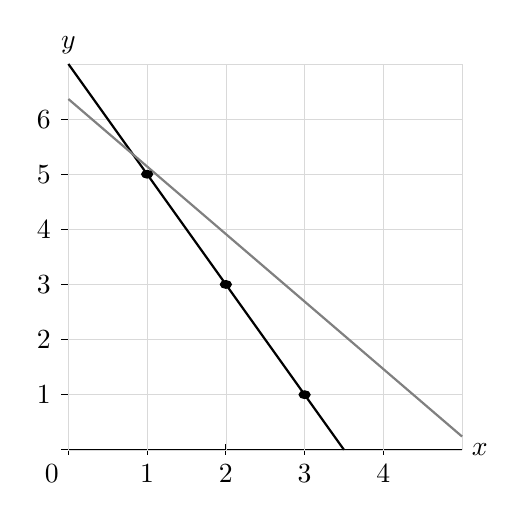
\begin{tikzpicture}[scale=1.0, xscale=1, yscale=0.7]
		\centering
		\draw (0,0) -- (5,0) node[right] {\(x\)};
		\draw (0,0) -- (0,7) node[above] {\(y\)};
		% Add tick marks (optional)

		\foreach \x in {1,2,3,4}
			\draw (\x,0.1) -- (\x,-0.1) node[below] {\x};

		\foreach \y in {1,2,3,4,5,6}
			\draw (0.1,\y) -- (-0.1,\y) node[left] {\y};

		\draw (0,0.1) -- (0, -0.1) node[below left] {0};
		\draw (0.1,0) -- (-0.1, 0) node[below left] {};

		\draw[very thin, gray!30] (0,0) grid (5,7);

		\draw[thick, black, domain=0:3.5] plot (\x, {7 - 2*\x}) node[right] {};
		\draw[thick, gray, domain=0:5.0] plot (\x, {9/sqrt(2) - sqrt(1.5)*\x}) node[right] {};

		\filldraw[black] (3,1) circle (2pt) node[below right] {};
		\filldraw[black] (2,3) circle (2pt) node[above right] {};
		\filldraw[black] (1,5) circle (2pt) node[above left] {};
	\end{tikzpicture}
	\caption{Representación de una capa entera (en negro) junto a un hiperplano afino que no es capa
	entera (en gris). La capa entera tiene como parámetros $\vec{v} = (2, 1)^T$ y $t = 1.4$,
	mientras que los del hiperplano afino son $\vec{v} = (\sqrt{3}, \sqrt{2})^T$ y $t = 1.4$.}
	\label{phase-1:fig:c-layer}
\end{figure}

Cualquier vector coprimo induce una familia de capas enteras y, sorprendentemente, esa familia
contiene a todos los puntos enteros en el espacio, como lo indica el siguiente teorema.

\begin{lemma}[\cite{herr}]
	Sean $\vec{v}, \vec{x} \in \R^n$ con $\vec{v}$ distinto de cero. Entonces $\vec{x} \in
	H_{\vec{v}, t_{\vec{x}}}$, donde $t_{\vec{x}} \coloneq \frac{\vec{v}^T\vec{x}}{\norm{\vec{v}}^2}$.
\end{lemma}

\begin{theorem}[\cite{herr}]
	Sea $\vec{v} \in \R^n$ un vector esencialmente entero y sea $\vec{w}$ su múltiplo coprimo.
	Entonces la familir de capas enteras $\left\lbrace H_{\vec{w}, k\norm{\vec{w}}^{-2}} \vcentcolon k
			\in \Z \right\rbrace$ cubre a $\Z^n$.
\end{theorem}
\begin{proof}
	% XXX: poner la demostración (?)
\end{proof}

% \begin{theorem}
% 	Sea $\vec{v} \in \R^n$ un vector esencialmente entero y sea $u \in \R$ un escalar. Entonces el
% 	número de capas enteras $\eta$ entre 0 y $u$ está determinado por
% 	\begin{equation}
% 		\eta = \left\lfloor
% 			u \cdot \frac{\lcm{\vec{v}_1, \ldots, \vec{v}_n}}{\gcd{\vec{v}_1, \ldots, \vec{v}_n}}
% 			\right\rfloor
% 	\end{equation}
% 	si $u \geq 0$. En caso de que $u$ sea negativo, tenemos
% 	\begin{equation}
% 		\eta = \left\lceil
% 			u \cdot \frac{\lcm{\vec{v}_1, \ldots, \vec{v}_n}}{\gcd{\vec{v}_1, \ldots, \vec{v}_n}}
% 			\right\rceil
% 	\end{equation}
% \end{theorem}
% \begin{proof}
% 	% TODO: demostrar el caso cuando u \geq 0, el otro es similar.
% \end{proof}

\section{Fase 1: una restricción presupuestaria}

\noindent
Sea $\vec{p} \in \R^n$ un vector esencialmente entero y sea $\vec{q} \in \Z^n$ su múltiplo coprimo.
Consideremos el programa lineal 
\begin{subequations}
	\label{phase-1:formulation}
	\begin{align}
		\max_{\vec{x} \in \R^n} \quad
			& \vec{p}^T\vec{x}, \label{phase-1:formulation:obj} \\
		\text{s.a.} \quad
			& \vec{p}^T\vec{x} \geq u, \label{phase-1:formulation:c_1} \\
			& \vec{x} \in \Z_{\geq 0}^n. \nonumber
	\end{align}
\end{subequations}

\section{Fase 2: múltiples restricciones junto con la presupuestaria}
\subsection{Estrategias alternativas para el problema de factibilidad}
\section{Fase 3: múltiples restricciones}
\section{Consideraciones y extensiones del algoritmo}
